
\documentclass{article}
% Define own Colorsceme 
\usepackage[dvipsnames]{xcolor}
% Change the colours if you want to
\definecolor{SlateGrey}{HTML}{2E2E2E}
\definecolor{LightGrey}{HTML}{666666}
\definecolor{DarkPastelRed}{HTML}{450808}
\definecolor{PastelRed}{HTML}{8F0D0D}
\definecolor{GoldenEarth}{HTML}{E7D192}
\definecolor{TextmarkerGreen}{HTML}{9DEF61}
\definecolor{TextmarkerRed}{HTML}{FF6085}
% Define own geometry
\usepackage[left=1.25cm,right=1.25cm,top=0.5cm,bottom=1.5cm, includehead, headheight=2cm]{geometry}

% build own logo
\usepackage{tikz}
% Build own header
\usepackage{fancyhdr}
% HEADER AND FOOTER
\pagestyle{fancy}  % Set Page Style (Header and Footer Style)
% Header
\fancyhead{} % Clears all default settings of the header 

\fancyhead{
\begin{tikzpicture}
\fill[SlateGrey] (0,0) rectangle (3,2);
\node[inner sep=0pt] (logo) at (1.5,1){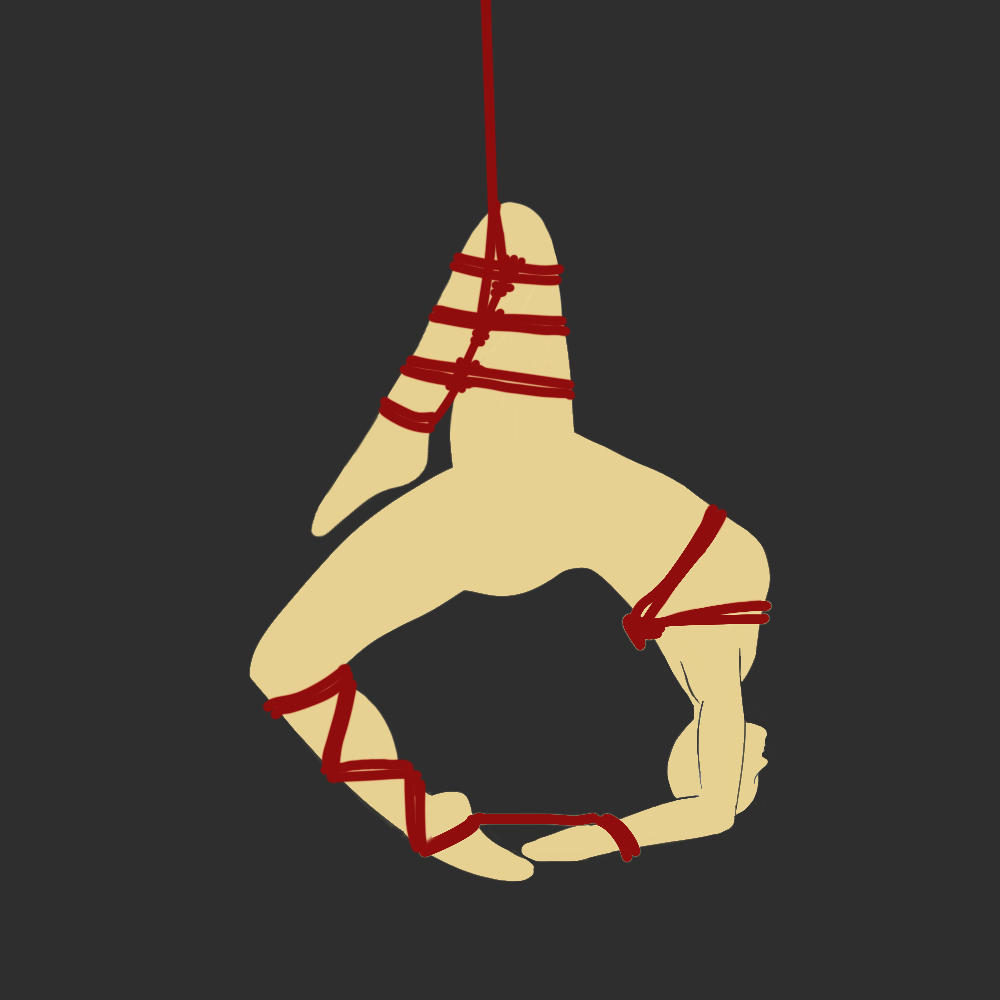
\includegraphics[width = 18mm]{logo.png}};
\fill[GoldenEarth] (3,0) rectangle (19.1,2);
\node[text centered] at (10,1.3) {\LARGE\textbf{Psychosoziale Hilfe}};
\node[text centered] at (10,0.7) {\large{Angebote ...}};
\node[text centered] at (18,1){\thepage};
\end{tikzpicture}
}
\fancyfoot{}
%\fancyhead[C]{\textbf{Code of Conduct}}
%\fancyhead[R]{\thepage}
\renewcommand{\headrulewidth}{0pt}  % Removes the default Horizontal Line in Header
\title{Psychosoziale Hilfe}
\author{Cato, Philomena und Mistbiene}


\begin{document}

Du entscheidest wann und in welcher Form du Unterstützung annehmen möchtest.
\\
\subsection*{Was wir anbieten möchten:}
\begin{itemize}
    \item Es steht ein großer Ruheraum zur allgemeinen Verfügung. Dieser kann jederzeit und von jeder Person in Anspruch genommen werden.
    \item Falls du dich unwohl fühlst steht eine Ansprechperson zur Verfügung, die dich auf deinen Wunsch unterstützt.
    \item Falls du dich unwohl fühlst steht eine Ansprechperson zur Verfügung, die dich auf deinen Wunsch unterstützt. Die Ansprechperson ist dafür da dich zu unterstützen, das Angebot richtet sich nach deinen Bedürfnissen
    \item Gespräche sind, soweit nicht anders mit dir vereinbart, vertraulich
    \item auf deinen Wunsch kann die Ansprechperson an die Orga oder andere Personen herantreten
deine Wahrnehmung und dein Erleben werden ernst genommen und anerkannt
\end{itemize}

\subsection*{Was wir explizit nicht anbieten:}
\begin{itemize}
    \item Beratung zu mittel- bis längerfristig bestehenden (u.a. psychischen) Problemen
    \item Entscheidungen im Bezug auf die Veranstaltung werden ausschließlich durch die Orga getroffen
    \item Es werden keine Beurteilung oder Bewertungen anderer Personen stattfinden
    \item Probleme zwischen Teilnehmenden lösen
\end{itemize}
\subsection*{Grenzen}
Alle am Workshop beteiligten Personen handeln im Rahmen ihrer persönlichen Möglichkeiten und Grenzen und achten darauf diese zu wahren. Wir machen das nicht hauptberuflich und haben keine professionelle psychologische Ausbildung.

\end{document}
